% ------------------------------------------------------------------------------
% TYPO3 Version 10.3 - What's New (Serbian Version)
%
% @license	Creative Commons BY-NC-SA 3.0
% @link		https://typo3.org/help/documentation/whats-new/
% @language	Serbian
% ------------------------------------------------------------------------------

\section{Sigurnost i privatnost}
\begin{frame}[fragile]
	\frametitle{Sigurnost i privatnost}

	\begin{center}\huge{Poglavlje 5:}\end{center}
	\begin{center}\huge{\color{typo3darkgrey}\textbf{Sigurnost i privatnost}}\end{center}

\end{frame}

% ------------------------------------------------------------------------------
% Feature | 90333 | Dashboard

\begin{frame}[fragile]
	\frametitle{Sigurnost i privatnost}
	\framesubtitle{Dashboard}

	\begin{itemize}
		\item Vidžeti sa Dashboard-a mogu da sadrže osetljive informacije.
		\item Stoga, preporuka je da se ograniči pristup vidžetima na bazi grupa.
		\item Korisnici administratorskog interfejsa imaju pristup samo vidžetima koji su im dostupni.
		\item Korisnik sa administratorskim privilegijama uvek ima pristup svim vidžetima.
	\end{itemize}

\end{frame}

% ------------------------------------------------------------------------------
% Feature | 89978 | Introduce Status Report for insecure exception handler settings

\begin{frame}[fragile]
	\frametitle{Sigurnost i privatnost}
	\framesubtitle{Statusni izveštaji}

	\begin{itemize}
		\item DebugExceptionHandler može da ispiše osetljive podatke koji mogu da
		 	uzrokuju povredu poverljivih informacija.
		\item Implementiran je novi statusni izveštaj da upozori administratore.
	\end{itemize}

	\vspace{0.4cm}
	\textbf{WARNING}, ukoliko je kontekst aplikacije podešen kao \textbf{development} i omogućeno je ispisivanje grešaka:
	\begin{figure}
		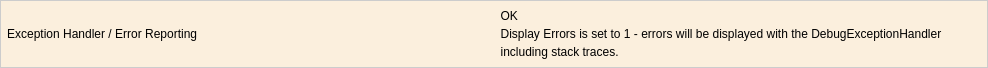
\includegraphics[width=1\linewidth]{SecurityAndPrivacy/89978a-IntroduceStatusReportForInsecureExceptionHandlerSettings.png}
	\end{figure}

	\textbf{ERROR}, ukoliko je kontekst aplikacije podešen kao \textbf{production} i omogućeno je ispisivanje grešaka:
	\begin{figure}
		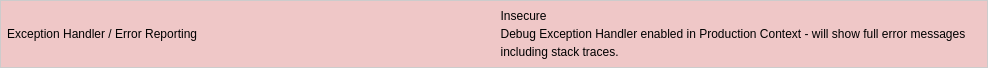
\includegraphics[width=1\linewidth]{SecurityAndPrivacy/89978b-IntroduceStatusReportForInsecureExceptionHandlerSettings.png}
	\end{figure}

\end{frame}

% ------------------------------------------------------------------------------
% Feature | 90351 | Allow TYPO3 to make SameSite cookies configurable

\begin{frame}[fragile]
	\frametitle{Sigurnost i privatnost}
	\framesubtitle{SameSite Cookies (1)}

	\begin{itemize}
		\item Za potrebe sigurnosti i privatnosti, od sada TYPO3 podržava opciju "SameSite"
			za kolačiće koje postavlja jezgro TYPO3.
		\item Ovaj atribut je podržan od strane većine modernih pretraživača i omogućava internet prezentacijama
			da definišu da li kolačići treba da budu ograničeni.
		\item Prema
			\href{https://www.owasp.org/index.php/SameSite}{OWASP}, SameSite kolačići\newline
			\small
				"\textit{smanjuju rizik za cross-origin curenje informacija}", sa\newline
				"\textit{dodatnom zaštitom od napada putem krivotvorenih zahteva sa drugih internet prezentacija}".
			\normalsize

		\item Validna podešavanja su "\textbf{strict}", "\textbf{lax}", ili \textit{not set}.
	\end{itemize}

\end{frame}

% ------------------------------------------------------------------------------
% Feature | 90351 | Allow TYPO3 to make SameSite cookies configurable

\begin{frame}[fragile]
	\frametitle{Sigurnost i privatnost}
	\framesubtitle{SameSite Cookies (2)}

	\begin{itemize}
		\item TYPO3 postavlja sledeće opcije:

			\begin{itemize}\small
				\item Sesija korisnickog interfejsa: "lax" kao podrazumevano podešavanje
				\item Sesija administratorskog interfejsa: "strict" kao podrazumevano podešavanje
				\item Install Tool sesija: "strict" (ne može se menjati)
				\item Last login provider (administratorski interfejs): "strict" (ne može se menjati)
			\end{itemize}\normalsize

		\item Install Tool poseduje konfiguraciju da se podesi politika
			SameSite kolačića u slučaju da su podrazumevana podešavanja previše stroga
			(na primer za autentifikaciju koja koristi OpenID/OAuth).

		\item Više o SameSite kolačićima možete pročitati u
			\href{https://tools.ietf.org/html/draft-ietf-httpbis-cookie-same-site-00}{RFC6265} (draft).
	\end{itemize}

\end{frame}

% ------------------------------------------------------------------------------
% Feature | 90262 | Add Argon2id to password hash algorithms

\begin{frame}[fragile]
	\frametitle{Sigurnost i privatnost}
	\framesubtitle{Algoritmi za hešovanje lozinki}

	\begin{itemize}
		\item Algoritam \texttt{Argon2i} ("i") je uveden sa TYPO3 v9 LTS.
		\item \texttt{Argon2id} ("id") je od sada takodje dostupan u TYPO3 pod uslovom da ga PHP podržava.
		\item \texttt{Argon2id} je hibrid nastao od \texttt{Argon2i} i \texttt{Argon2d}
			i dosta je otporniji na napade.
		\item \texttt{Argon2id} je dostupan na sistemima sa PHP verzijom 7.3 ili većom.
	\end{itemize}

\end{frame}

% ------------------------------------------------------------------------------
